\documentclass[10pt,a4paper]{report}
\usepackage[utf8]{inputenc}
\usepackage{amsmath}
\usepackage{amsfonts}
\usepackage{amssymb}
\usepackage{amsthm}
\usepackage{hyperref}

\usepackage{multicol}
\usepackage{fancyhdr}
\usepackage[inline]{enumitem}
\usepackage{tikz}
\usepackage{tikz-cd}
\usetikzlibrary{calc}
\usetikzlibrary{shapes.geometric}
\usepackage[margin=0.5in]{geometry}
\usepackage{xcolor}
\usepackage{ esint }

\hypersetup{
    colorlinks=true,
    linkcolor=blue,
    filecolor=magenta,      
    urlcolor=cyan,
    pdftitle={Tensors},
    pdfpagemode=FullScreen,
    }

%\urlstyle{same}

\newcommand{\CLASSNAME}{Math 5230 -- Partial Differential Equations}
\newcommand{\STUDENTNAME}{Paul Carmody}
\newcommand{\ASSIGNMENT}{Homework \#5 }
\newcommand{\DUEDATE}{December 1, 2025}
\newcommand{\SEMESTER}{Fall 2025}
\newcommand{\SCHEDULE}{MW 2:00 -- 3:15}
\newcommand{\ROOM}{Crawford 332}

\newcommand{\MMN}{M_{m\times n}}
\newcommand{\FF}{\mathcal{F}}

\pagestyle{fancy}
\fancyhf{}
\chead{ \fancyplain{}{\CLASSNAME} }
%\chead{ \fancyplain{}{\STUDENTNAME} }
\rhead{\thepage}
\input{../MyMacros}

\newcommand{\RED}[1]{\textcolor{red}{#1}}
\newcommand{\BLUE}[1]{\textcolor{blue}{#1}}

\newcommand{\CURL}{\operatorname{curl}}
\newcommand{\DIV}{\operatorname{div}}

\begin{document}

\begin{center}
	\Large{\CLASSNAME -- \SEMESTER} \\
	\large{ w/Professor Snelson}
\end{center}
\begin{center}
	\STUDENTNAME \\
	\ASSIGNMENT -- \DUEDATE\\
\end{center} 

\noindent Please show your work and justify all answers.

\begin{enumerate}

\item Use the method of characteristics to solve the initial value problem 
\begin{align*}
	\BINDEF{u_t+xu_x = 2tu, & x \in \R, t>0}{u(x,0)=g(x)}
\end{align*}
%see page 117

\BLUE{Thus, $\frac{dt}{ds}=1$, $\frac{dx}{ds}=x$ and $\frac{du}{ds}=-2t u$  Then
\begin{align*}
	t(s) &= s,\, x(s)=Ce^s \implies x(t)= Ce^t
\end{align*}or $C = xe^{-t}$.  Now $\frac{du}{ds} = 2su$.  Thus, $u = De^{s^2}=De^{t^2}$ and since $u(0,0) = g(0) = Ce^0 = C$, $D=C$.  Or $u(x,t) = g(C)e^{t^2} = g(xe^{-t})e^{t^2}$
}

\item Write down a linear transport equation of the form
\begin{align*}
	a(x,t)u_t+b(x,t)u_x = 0
\end{align*}so that the characteristic curves $(x(s), t(s))$ are parabolas.  (In other words, you need to say what $a(x,t)$ and $b(x,t)$ are.)  You do not need to find the solution $u(x,t)$.

\BLUE{We may start with $\frac{dt}{ds} = a(x,t)$ and $\frac{dx}{ds}=b(x,t)$.  Also, we want $x = Ct^2$.  Thus, at any given point $\frac{dx}{dt}=2Ct$.  Thus, the characteristic slope is $C = \frac{x}{t^2}$ or $\frac{dx}{dt}= 2Ct=2\PAREN{\frac{x}{t^2}}t=\frac{2x}{t}$.  Thus, $\frac{b(x,t)}{a(x,t)}=\frac{2x}{t}$ or 
\begin{align*}
	a(x,t) &= t & \quad &\AND & \quad b(x,t) = 2x
\end{align*}
}

\item Use the method of characteristics to solve the initial value problem
\begin{align*}
	\BINDEF{u_t+\PAREN{\frac{1}{3}u^3}_x = 0, & x\in \R, t>0,}{u(x,0)=g(x)}
\end{align*}where
\begin{align*}
	g(x) &= \BINDEF{1,&x<0}{0,&x\ge 0}
\end{align*}(Hint: The problem features a shock.  Use the jump conditions to determine the path of the shock.)

\BLUE{Rewrite the expression in terms of $u_x$
\begin{align*}
	u_t+\PAREN{\frac{1}{3}u^3}_x &= u_t+u^2u_x 
\end{align*}hence the characteristic speed is $f'(u) = u^2$ which depends on $u$, thus, generate a shock.  Defining
\begin{align*}
	f(u_L) &=  1/3 \text{ for } x<0 \AND f(u_R) = 0 \text{ for } x\ge 0 
\end{align*}these are then used in the Rankin-Hugoniot condition as 
\begin{align*}
	s= \frac{f(u_R)-f(u_L)}{u_R-u_L} &= \frac{0-1/3}{0-1} = \frac{1}{3}
\end{align*}Further, we must have that  $f'(u_L) > s > f'(u_R)$, thus $(f'(1) = 1) > (s=1/3) > (f'(0)=0)$, which is true.  Therefore, 
\begin{align*}
	u(x,t) &= \BINDEF{1, & x < \frac{1}{3}t}{0, & x > \frac{1}{3}t}
\end{align*}
}

\item Consider the same PDE from probem 4, with intial data
\begin{align*}
	g(x) &= \BINDEF{1,&x<0}{0,&x\ge 0}
\end{align*}Find a solution to this problem that has no shocks, i.e., the solution is continuous for positive times.  The solution will look like a fan-shaped rarefaction wave.

\BLUE{The PDE from problem 4 is 
\begin{align*}
	u_t-\textbf{b}\cdot Du = f \in \R^n \times (0,\infty),
\end{align*}where $\textbf{b}\in \R^n, f=f(x,t)$. This is a non-homogenous Transport Equation so the solution is 
\begin{align*}
	u(x,t) &= g(x+bt) + \int_0^t f(x+b(t-\tau), \tau)\, d\tau
\end{align*}
}

\item Verify by direct calculation that 
\begin{align*}
	u(x,t) = \BINDEF{0, &x< t/2}{1,&x\ge t/s}
\end{align*}is pointwise solution to the initial value problem from problem 5, at every point except the line of discontinuity $x = t/2$.

Explain why this shock (discontinuity) is non-physical.  Check that the entropy condition $F'(u_l)>\sigma>F'(u_r)$ is not staisfied.

\BLUE{The initial value problem is problem 5(b)
\begin{align*}
	x_1u_{x_1}+2x_2(u_{x_2})+u_{x_3} = 3u,\, u(x_1,x_2,0) = g(x_1,x_2).
\end{align*}
}Verify by direct calculation that 
\begin{align*}
	u(x,t) = \BINDEF{0, &x< t/2}{1,&x\ge t/s}
\end{align*}is pointwise solution to the initial value problem \begin{align*}
	x_1u_{x_1}+2x_2(u_{x_2})+u_{x_3} = 3u,\, u(x_1,x_2,0) = g(x_1,x_2).
\end{align*}, at every point except the line of discontinuity $x = t/2$.
Explain why this shock (discontinuity) is non-physical.  Check that the entropy condition $F'(u_l)>\sigma>F'(u_r)$ is not staisfied.


\newpage
\item Recall that a linear second-order PDE
\begin{align*}
	Au_{xx}+Bu_{xy}+Cu_{yy}+Du_x+Eu_y+Fu=0
\end{align*}is \textit{elliptic} if $B^2< 4AC$, \textit{hyperbolic} if $B^2>4AC$, and \textit{parabolic} if $B^2 = 4AC$.
\begin{enumerate}
	\item Classify the following two PDEs:
	\begin{align*}
		u_{xx}-u_{xy}+2u_y+u_{yy}-3u_{yx}-4u&=0\\
		9u_{xx}+6_{xy}+y_{yy}+u_x&=0
	\end{align*}
	
	\item Find the regions in the $xy$ plane where the equation
	\begin{align*}
		(1+x)u_{xx}+2xyu_{xy}-y^2u_{yy}=0
	\end{align*}is elliptic, hyperbolic, or parabolic.  Sketch them.
	\end{enumerate}
	
	\BLUE{First, $A=1+x, B=2xy, C=-y^2$.  Thus, the discrimant, $D$ is
	\begin{align*}
		 D = B^2-4AC &= (2xy)^2-4(1+x)(-y^2)
\end{align*}	thus $D=0$
\begin{align*}
	4x^2y^2&=4(1+x)y^2 \\
	x^2y^2&=(1+x)y^2 \\
	x^2&=-(1+x) \\
	x^2-x-1 &= 0
\end{align*}
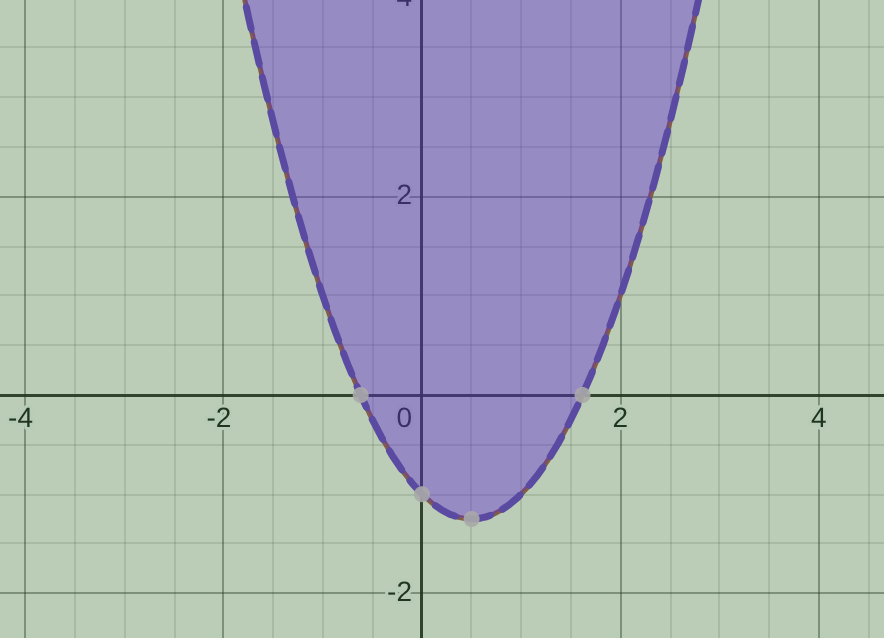
\includegraphics[scale=0.4]{Homework_5.png} \\
where $D>0$, the purple area, is hyperbolic, when $D<0$, the green area, is elliptic and when $D=0$, the border between them, is parabolic.
	}

\end{enumerate}

\end{document}
